\documentclass[twoside]{book}

% Packages required by doxygen
\usepackage{fixltx2e}
\usepackage{calc}
\usepackage{doxygen}
\usepackage[export]{adjustbox} % also loads graphicx
\usepackage{graphicx}
\usepackage[utf8]{inputenc}
\usepackage{makeidx}
\usepackage{multicol}
\usepackage{multirow}
\PassOptionsToPackage{warn}{textcomp}
\usepackage{textcomp}
\usepackage[nointegrals]{wasysym}
\usepackage[table]{xcolor}

% Font selection
\usepackage[T1]{fontenc}
\usepackage[scaled=.90]{helvet}
\usepackage{courier}
\usepackage{amssymb}
\usepackage{sectsty}
\renewcommand{\familydefault}{\sfdefault}
\allsectionsfont{%
  \fontseries{bc}\selectfont%
  \color{darkgray}%
}
\renewcommand{\DoxyLabelFont}{%
  \fontseries{bc}\selectfont%
  \color{darkgray}%
}
\newcommand{\+}{\discretionary{\mbox{\scriptsize$\hookleftarrow$}}{}{}}

% Page & text layout
\usepackage{geometry}
\geometry{%
  a4paper,%
  top=2.5cm,%
  bottom=2.5cm,%
  left=2.5cm,%
  right=2.5cm%
}
\tolerance=750
\hfuzz=15pt
\hbadness=750
\setlength{\emergencystretch}{15pt}
\setlength{\parindent}{0cm}
\setlength{\parskip}{0.2cm}
\makeatletter
\renewcommand{\paragraph}{%
  \@startsection{paragraph}{4}{0ex}{-1.0ex}{1.0ex}{%
    \normalfont\normalsize\bfseries\SS@parafont%
  }%
}
\renewcommand{\subparagraph}{%
  \@startsection{subparagraph}{5}{0ex}{-1.0ex}{1.0ex}{%
    \normalfont\normalsize\bfseries\SS@subparafont%
  }%
}
\makeatother

% Headers & footers
\usepackage{fancyhdr}
\pagestyle{fancyplain}
\fancyhead[LE]{\fancyplain{}{\bfseries\thepage}}
\fancyhead[CE]{\fancyplain{}{}}
\fancyhead[RE]{\fancyplain{}{\bfseries\leftmark}}
\fancyhead[LO]{\fancyplain{}{\bfseries\rightmark}}
\fancyhead[CO]{\fancyplain{}{}}
\fancyhead[RO]{\fancyplain{}{\bfseries\thepage}}
\fancyfoot[LE]{\fancyplain{}{}}
\fancyfoot[CE]{\fancyplain{}{}}
\fancyfoot[RE]{\fancyplain{}{\bfseries\scriptsize Generated on Tue Nov 17 2015 16\+:02\+:05 for Assignment 2 by Doxygen }}
\fancyfoot[LO]{\fancyplain{}{\bfseries\scriptsize Generated on Tue Nov 17 2015 16\+:02\+:05 for Assignment 2 by Doxygen }}
\fancyfoot[CO]{\fancyplain{}{}}
\fancyfoot[RO]{\fancyplain{}{}}
\renewcommand{\footrulewidth}{0.4pt}
\renewcommand{\chaptermark}[1]{%
  \markboth{#1}{}%
}
\renewcommand{\sectionmark}[1]{%
  \markright{\thesection\ #1}%
}

% Indices & bibliography
\usepackage{natbib}
\usepackage[titles]{tocloft}
\setcounter{tocdepth}{3}
\setcounter{secnumdepth}{5}
\makeindex

% Hyperlinks (required, but should be loaded last)
\usepackage{ifpdf}
\ifpdf
  \usepackage[pdftex,pagebackref=true]{hyperref}
\else
  \usepackage[ps2pdf,pagebackref=true]{hyperref}
\fi
\hypersetup{%
  colorlinks=true,%
  linkcolor=blue,%
  citecolor=blue,%
  unicode%
}

% Custom commands
\newcommand{\clearemptydoublepage}{%
  \newpage{\pagestyle{empty}\cleardoublepage}%
}


%===== C O N T E N T S =====

\begin{document}

% Titlepage & ToC
\hypersetup{pageanchor=false,
             bookmarks=true,
             bookmarksnumbered=true,
             pdfencoding=unicode
            }
\pagenumbering{roman}
\begin{titlepage}
\vspace*{7cm}
\begin{center}%
{\Large Assignment 2 }\\
\vspace*{1cm}
{\large Generated by Doxygen 1.8.10}\\
\vspace*{0.5cm}
{\small Tue Nov 17 2015 16:02:05}\\
\end{center}
\end{titlepage}
\clearemptydoublepage
\tableofcontents
\clearemptydoublepage
\pagenumbering{arabic}
\hypersetup{pageanchor=true}

%--- Begin generated contents ---
\chapter{Installing}
\label{md__i_n_s_t_a_l_l}
\hypertarget{md__i_n_s_t_a_l_l}{}
Generating the documentation can be done by\+:


\begin{DoxyCode}
1 $ pdflatex document.tex
\end{DoxyCode}
 
\chapter{S\+E\+N\+G-\/330}
\label{md__r_e_a_d_m_e}
\hypertarget{md__r_e_a_d_m_e}{}
Uvic S\+E\+N\+G 330 201509 
\chapter{Namespace Index}
\section{Namespace List}
Here is a list of all namespaces with brief descriptions\+:\begin{DoxyCompactList}
\item\contentsline{section}{\hyperlink{namespaceenemy}{enemy} }{\pageref{namespaceenemy}}{}
\end{DoxyCompactList}

\chapter{Hierarchical Index}
\section{Class Hierarchy}
This inheritance list is sorted roughly, but not completely, alphabetically\+:\begin{DoxyCompactList}
\item \contentsline{section}{Driver}{\pageref{class_driver}}{}
\item \contentsline{section}{enemy.\+Enemy}{\pageref{classenemy_1_1_enemy}}{}
\item \contentsline{section}{Game}{\pageref{class_game}}{}
\item \contentsline{section}{Game\+Object}{\pageref{class_game_object}}{}
\begin{DoxyCompactList}
\item \contentsline{section}{Adversary}{\pageref{class_adversary}}{}
\end{DoxyCompactList}
\item Message\+Or\+Builder\begin{DoxyCompactList}
\item \contentsline{section}{enemy.\+Enemy.\+Monster\+Or\+Builder}{\pageref{interfaceenemy_1_1_enemy_1_1_monster_or_builder}}{}
\item \contentsline{section}{enemy.\+Enemy.\+Trap\+Or\+Builder}{\pageref{interfaceenemy_1_1_enemy_1_1_trap_or_builder}}{}
\end{DoxyCompactList}
\item \contentsline{section}{Player}{\pageref{class_player}}{}
\item \contentsline{section}{Room}{\pageref{class_room}}{}
\item \contentsline{section}{Test\+Bed1}{\pageref{class_test_bed1}}{}
\item \contentsline{section}{Test\+Cases}{\pageref{class_test_cases}}{}
\end{DoxyCompactList}

\chapter{Class Index}
\section{Class List}
Here are the classes, structs, unions and interfaces with brief descriptions\+:\begin{DoxyCompactList}
\item\contentsline{section}{\hyperlink{class_adversary}{Adversary} }{\pageref{class_adversary}}{}
\item\contentsline{section}{\hyperlink{class_driver}{Driver} }{\pageref{class_driver}}{}
\item\contentsline{section}{\hyperlink{classenemy_1_1_enemy}{enemy.\+Enemy} }{\pageref{classenemy_1_1_enemy}}{}
\item\contentsline{section}{\hyperlink{class_game}{Game} }{\pageref{class_game}}{}
\item\contentsline{section}{\hyperlink{class_game_object}{Game\+Object} }{\pageref{class_game_object}}{}
\item\contentsline{section}{\hyperlink{interfaceenemy_1_1_enemy_1_1_monster_or_builder}{enemy.\+Enemy.\+Monster\+Or\+Builder} }{\pageref{interfaceenemy_1_1_enemy_1_1_monster_or_builder}}{}
\item\contentsline{section}{\hyperlink{class_player}{Player} }{\pageref{class_player}}{}
\item\contentsline{section}{\hyperlink{class_room}{Room} }{\pageref{class_room}}{}
\item\contentsline{section}{\hyperlink{class_test_bed1}{Test\+Bed1} }{\pageref{class_test_bed1}}{}
\item\contentsline{section}{\hyperlink{class_test_cases}{Test\+Cases} }{\pageref{class_test_cases}}{}
\item\contentsline{section}{\hyperlink{interfaceenemy_1_1_enemy_1_1_trap_or_builder}{enemy.\+Enemy.\+Trap\+Or\+Builder} }{\pageref{interfaceenemy_1_1_enemy_1_1_trap_or_builder}}{}
\end{DoxyCompactList}

\chapter{File Index}
\section{File List}
Here is a list of all files with brief descriptions\+:\begin{DoxyCompactList}
\item\contentsline{section}{other/project\+\_\+phase3/\hyperlink{other_2project__phase3_2_room_8java}{Room.\+java} }{\pageref{other_2project__phase3_2_room_8java}}{}
\item\contentsline{section}{src/\hyperlink{_adversary_8java}{Adversary.\+java} }{\pageref{_adversary_8java}}{}
\item\contentsline{section}{src/\hyperlink{_driver_8java}{Driver.\+java} }{\pageref{_driver_8java}}{}
\item\contentsline{section}{src/\hyperlink{_game_8java}{Game.\+java} }{\pageref{_game_8java}}{}
\item\contentsline{section}{src/\hyperlink{_game_object_8java}{Game\+Object.\+java} }{\pageref{_game_object_8java}}{}
\item\contentsline{section}{src/\hyperlink{_player_8java}{Player.\+java} }{\pageref{_player_8java}}{}
\item\contentsline{section}{src/\hyperlink{src_2_room_8java}{Room.\+java} }{\pageref{src_2_room_8java}}{}
\item\contentsline{section}{src/\hyperlink{_test_bed1_8java}{Test\+Bed1.\+java} }{\pageref{_test_bed1_8java}}{}
\item\contentsline{section}{src/\hyperlink{_test_cases_8java}{Test\+Cases.\+java} }{\pageref{_test_cases_8java}}{}
\item\contentsline{section}{src/\hyperlink{_world_builder_8java}{World\+Builder.\+java} }{\pageref{_world_builder_8java}}{}
\item\contentsline{section}{src/protobuf/\hyperlink{_enemy_8java}{Enemy.\+java} }{\pageref{_enemy_8java}}{}
\end{DoxyCompactList}

\chapter{Namespace Documentation}
\hypertarget{namespaceenemy}{}\section{Package enemy}
\label{namespaceenemy}\index{enemy@{enemy}}
\subsection*{Classes}
\begin{DoxyCompactItemize}
\item 
class \hyperlink{classenemy_1_1_enemy}{Enemy}
\end{DoxyCompactItemize}

\chapter{Class Documentation}
\hypertarget{class_adversary}{}\section{Adversary Class Reference}
\label{class_adversary}\index{Adversary@{Adversary}}
Inheritance diagram for Adversary\+:\begin{figure}[H]
\begin{center}
\leavevmode
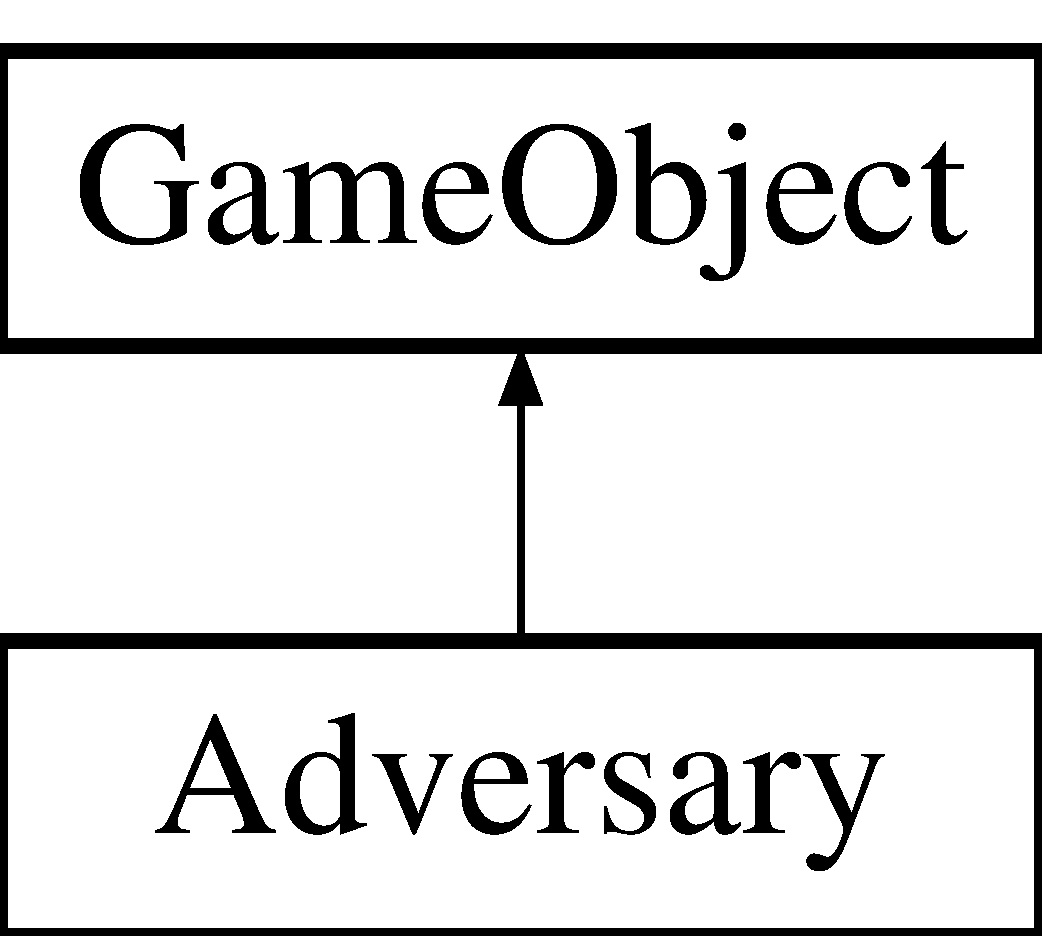
\includegraphics[height=2.000000cm]{class_adversary}
\end{center}
\end{figure}
\subsection*{Public Member Functions}
\begin{DoxyCompactItemize}
\item 
\hyperlink{class_adversary_af14ddd9652c9542b5b5900751dea5364}{Adversary} ()
\item 
\hyperlink{class_adversary_a208bf7c3fceb6d46dfd0020595810fff}{Adversary} (int h, int a)
\end{DoxyCompactItemize}
\subsection*{Static Public Member Functions}
\begin{DoxyCompactItemize}
\item 
static int \hyperlink{class_adversary_a717e855e0d76e1ca21d5e622515ac35e}{recieve\+Damage} (\hyperlink{class_player}{Player} p)
\end{DoxyCompactItemize}


\subsection{Detailed Description}
Extends game\+Object for the adversaries to interact with the player. The adversary can either be a monster or a trap. 

\subsection{Constructor \& Destructor Documentation}
\hypertarget{class_adversary_af14ddd9652c9542b5b5900751dea5364}{}\index{Adversary@{Adversary}!Adversary@{Adversary}}
\index{Adversary@{Adversary}!Adversary@{Adversary}}
\subsubsection[{Adversary()}]{\setlength{\rightskip}{0pt plus 5cm}Adversary.\+Adversary (
\begin{DoxyParamCaption}
{}
\end{DoxyParamCaption}
)\hspace{0.3cm}{\ttfamily [inline]}}\label{class_adversary_af14ddd9652c9542b5b5900751dea5364}
\hypertarget{class_adversary_a208bf7c3fceb6d46dfd0020595810fff}{}\index{Adversary@{Adversary}!Adversary@{Adversary}}
\index{Adversary@{Adversary}!Adversary@{Adversary}}
\subsubsection[{Adversary(int h, int a)}]{\setlength{\rightskip}{0pt plus 5cm}Adversary.\+Adversary (
\begin{DoxyParamCaption}
\item[{int}]{h, }
\item[{int}]{a}
\end{DoxyParamCaption}
)\hspace{0.3cm}{\ttfamily [inline]}}\label{class_adversary_a208bf7c3fceb6d46dfd0020595810fff}


\subsection{Member Function Documentation}
\hypertarget{class_adversary_a717e855e0d76e1ca21d5e622515ac35e}{}\index{Adversary@{Adversary}!recieve\+Damage@{recieve\+Damage}}
\index{recieve\+Damage@{recieve\+Damage}!Adversary@{Adversary}}
\subsubsection[{recieve\+Damage(\+Player p)}]{\setlength{\rightskip}{0pt plus 5cm}static int Adversary.\+recieve\+Damage (
\begin{DoxyParamCaption}
\item[{{\bf Player}}]{p}
\end{DoxyParamCaption}
)\hspace{0.3cm}{\ttfamily [inline]}, {\ttfamily [static]}}\label{class_adversary_a717e855e0d76e1ca21d5e622515ac35e}


The documentation for this class was generated from the following file\+:\begin{DoxyCompactItemize}
\item 
src/\hyperlink{_adversary_8java}{Adversary.\+java}\end{DoxyCompactItemize}

\hypertarget{class_driver}{}\section{Driver Class Reference}
\label{class_driver}\index{Driver@{Driver}}
\subsection*{Static Public Member Functions}
\begin{DoxyCompactItemize}
\item 
static void \hyperlink{class_driver_ad96bcac1144441cfe3fdf2e728349b79}{main} (String args\mbox{[}$\,$\mbox{]})  throws I\+O\+Exception 
\item 
static void \hyperlink{class_driver_aa89853174e62c333ae37e86bb3c32c60}{run\+Command} (String cmd, \hyperlink{class_game}{Game} g)
\end{DoxyCompactItemize}


\subsection{Detailed Description}
Main driver for the game, will create a game\+Object g and runs a loop to process commands from the console. 

\subsection{Member Function Documentation}
\hypertarget{class_driver_ad96bcac1144441cfe3fdf2e728349b79}{}\index{Driver@{Driver}!main@{main}}
\index{main@{main}!Driver@{Driver}}
\subsubsection[{main(\+String args[])}]{\setlength{\rightskip}{0pt plus 5cm}static void Driver.\+main (
\begin{DoxyParamCaption}
\item[{String}]{args\mbox{[}$\,$\mbox{]}}
\end{DoxyParamCaption}
) throws I\+O\+Exception\hspace{0.3cm}{\ttfamily [inline]}, {\ttfamily [static]}}\label{class_driver_ad96bcac1144441cfe3fdf2e728349b79}
\hypertarget{class_driver_aa89853174e62c333ae37e86bb3c32c60}{}\index{Driver@{Driver}!run\+Command@{run\+Command}}
\index{run\+Command@{run\+Command}!Driver@{Driver}}
\subsubsection[{run\+Command(\+String cmd, Game g)}]{\setlength{\rightskip}{0pt plus 5cm}static void Driver.\+run\+Command (
\begin{DoxyParamCaption}
\item[{String}]{cmd, }
\item[{{\bf Game}}]{g}
\end{DoxyParamCaption}
)\hspace{0.3cm}{\ttfamily [inline]}, {\ttfamily [static]}}\label{class_driver_aa89853174e62c333ae37e86bb3c32c60}
Contains the switches for the game to run and process command, all command from the Available commands are \char`\"{}help\char`\"{} \char`\"{}pick up items\char`\"{} fight monster\char`\"{}
\char`\"{}move room\char`\"{}
\char`\"{}check inventory\char`\"{}
\char`\"{}use item" 
\begin{DoxyParams}{Parameters}
{\em g} & \hyperlink{class_game}{Game} object game object created from \hyperlink{class_driver_ad96bcac1144441cfe3fdf2e728349b79}{main()} \\
\hline
{\em cmd} & command string taken from the console. \\
\hline
\end{DoxyParams}


The documentation for this class was generated from the following file\+:\begin{DoxyCompactItemize}
\item 
src/\hyperlink{_driver_8java}{Driver.\+java}\end{DoxyCompactItemize}

\hypertarget{classenemy_1_1_enemy}{}\section{enemy.\+Enemy Class Reference}
\label{classenemy_1_1_enemy}\index{enemy.\+Enemy@{enemy.\+Enemy}}
\subsection*{Classes}
\begin{DoxyCompactItemize}
\item 
class {\bfseries Monster}
\item 
interface \hyperlink{interfaceenemy_1_1_enemy_1_1_monster_or_builder}{Monster\+Or\+Builder}
\item 
class {\bfseries Trap}
\item 
interface \hyperlink{interfaceenemy_1_1_enemy_1_1_trap_or_builder}{Trap\+Or\+Builder}
\end{DoxyCompactItemize}
\subsection*{Static Public Member Functions}
\begin{DoxyCompactItemize}
\item 
static void \hyperlink{classenemy_1_1_enemy_aece4b94ff7a553cba559ea11dc4a593c}{register\+All\+Extensions} (com.\+google.\+protobuf.\+Extension\+Registry registry)
\item 
static com.\+google.\+protobuf.\+Descriptors.\+File\+Descriptor \hyperlink{classenemy_1_1_enemy_a9bff27ee4443d321a822f6e479469eea}{get\+Descriptor} ()
\end{DoxyCompactItemize}


\subsection{Member Function Documentation}
\hypertarget{classenemy_1_1_enemy_a9bff27ee4443d321a822f6e479469eea}{}\index{enemy\+::\+Enemy@{enemy\+::\+Enemy}!get\+Descriptor@{get\+Descriptor}}
\index{get\+Descriptor@{get\+Descriptor}!enemy\+::\+Enemy@{enemy\+::\+Enemy}}
\subsubsection[{get\+Descriptor()}]{\setlength{\rightskip}{0pt plus 5cm}static com.\+google.\+protobuf.\+Descriptors.\+File\+Descriptor enemy.\+Enemy.\+get\+Descriptor (
\begin{DoxyParamCaption}
{}
\end{DoxyParamCaption}
)\hspace{0.3cm}{\ttfamily [inline]}, {\ttfamily [static]}}\label{classenemy_1_1_enemy_a9bff27ee4443d321a822f6e479469eea}
\hypertarget{classenemy_1_1_enemy_aece4b94ff7a553cba559ea11dc4a593c}{}\index{enemy\+::\+Enemy@{enemy\+::\+Enemy}!register\+All\+Extensions@{register\+All\+Extensions}}
\index{register\+All\+Extensions@{register\+All\+Extensions}!enemy\+::\+Enemy@{enemy\+::\+Enemy}}
\subsubsection[{register\+All\+Extensions(com.\+google.\+protobuf.\+Extension\+Registry registry)}]{\setlength{\rightskip}{0pt plus 5cm}static void enemy.\+Enemy.\+register\+All\+Extensions (
\begin{DoxyParamCaption}
\item[{com.\+google.\+protobuf.\+Extension\+Registry}]{registry}
\end{DoxyParamCaption}
)\hspace{0.3cm}{\ttfamily [inline]}, {\ttfamily [static]}}\label{classenemy_1_1_enemy_aece4b94ff7a553cba559ea11dc4a593c}


The documentation for this class was generated from the following file\+:\begin{DoxyCompactItemize}
\item 
src/protobuf/\hyperlink{_enemy_8java}{Enemy.\+java}\end{DoxyCompactItemize}

\hypertarget{class_game}{}\section{Game Class Reference}
\label{class_game}\index{Game@{Game}}
\subsection*{Public Member Functions}
\begin{DoxyCompactItemize}
\item 
\hyperlink{class_game_a2e034e53e9c032964ecd2a831b29a616}{Game} ()
\item 
\hyperlink{class_game_a562ff3d3722644681c165b571c77e493}{Game} (int end\+Rooms)
\item 
boolean \hyperlink{class_game_a379992cc9373a228b47c7ed398fc82a3}{is\+Running} ()
\end{DoxyCompactItemize}
\subsection*{Public Attributes}
\begin{DoxyCompactItemize}
\item 
\hyperlink{class_player}{Player} \hyperlink{class_game_abca4659998fe751258381792e922f138}{player} = new \hyperlink{class_player}{Player}()
\item 
int \hyperlink{class_game_a6c971d217035a9afd591a2fef942593d}{current\+Rooms}
\item 
int \hyperlink{class_game_a35d7485500ee1c2ec4ec93201aebddbb}{max\+Rooms}
\end{DoxyCompactItemize}


\subsection{Detailed Description}
Creates a new player object(class constructor) for the game and while game is currently a placeholder for the game obect which will run the game. \begin{DoxyAuthor}{Author}
Breck Wagner 

Mook Tungs 

Zac Broitman 

Greg Bacic 
\end{DoxyAuthor}


\subsection{Constructor \& Destructor Documentation}
\hypertarget{class_game_a2e034e53e9c032964ecd2a831b29a616}{}\index{Game@{Game}!Game@{Game}}
\index{Game@{Game}!Game@{Game}}
\subsubsection[{Game()}]{\setlength{\rightskip}{0pt plus 5cm}Game.\+Game (
\begin{DoxyParamCaption}
{}
\end{DoxyParamCaption}
)\hspace{0.3cm}{\ttfamily [inline]}}\label{class_game_a2e034e53e9c032964ecd2a831b29a616}
Constructor for the game with static variables. \hypertarget{class_game_a562ff3d3722644681c165b571c77e493}{}\index{Game@{Game}!Game@{Game}}
\index{Game@{Game}!Game@{Game}}
\subsubsection[{Game(int end\+Rooms)}]{\setlength{\rightskip}{0pt plus 5cm}Game.\+Game (
\begin{DoxyParamCaption}
\item[{int}]{end\+Rooms}
\end{DoxyParamCaption}
)\hspace{0.3cm}{\ttfamily [inline]}}\label{class_game_a562ff3d3722644681c165b571c77e493}
Constructor for \hyperlink{class_game}{Game} with set number of end Rooms 
\begin{DoxyParams}{Parameters}
{\em end\+Rooms} & sets the last number of rooms before the game will end, with the player beating the game. \\
\hline
\end{DoxyParams}


\subsection{Member Function Documentation}
\hypertarget{class_game_a379992cc9373a228b47c7ed398fc82a3}{}\index{Game@{Game}!is\+Running@{is\+Running}}
\index{is\+Running@{is\+Running}!Game@{Game}}
\subsubsection[{is\+Running()}]{\setlength{\rightskip}{0pt plus 5cm}boolean Game.\+is\+Running (
\begin{DoxyParamCaption}
{}
\end{DoxyParamCaption}
)\hspace{0.3cm}{\ttfamily [inline]}}\label{class_game_a379992cc9373a228b47c7ed398fc82a3}
checks the pleayrs health while the game is running. \begin{DoxyReturn}{Returns}
boolean denoting wether the player objects health is greater than 0 
\end{DoxyReturn}


\subsection{Member Data Documentation}
\hypertarget{class_game_a6c971d217035a9afd591a2fef942593d}{}\index{Game@{Game}!current\+Rooms@{current\+Rooms}}
\index{current\+Rooms@{current\+Rooms}!Game@{Game}}
\subsubsection[{current\+Rooms}]{\setlength{\rightskip}{0pt plus 5cm}int Game.\+current\+Rooms}\label{class_game_a6c971d217035a9afd591a2fef942593d}
\hypertarget{class_game_a35d7485500ee1c2ec4ec93201aebddbb}{}\index{Game@{Game}!max\+Rooms@{max\+Rooms}}
\index{max\+Rooms@{max\+Rooms}!Game@{Game}}
\subsubsection[{max\+Rooms}]{\setlength{\rightskip}{0pt plus 5cm}int Game.\+max\+Rooms}\label{class_game_a35d7485500ee1c2ec4ec93201aebddbb}
\hypertarget{class_game_abca4659998fe751258381792e922f138}{}\index{Game@{Game}!player@{player}}
\index{player@{player}!Game@{Game}}
\subsubsection[{player}]{\setlength{\rightskip}{0pt plus 5cm}{\bf Player} Game.\+player = new {\bf Player}()}\label{class_game_abca4659998fe751258381792e922f138}


The documentation for this class was generated from the following file\+:\begin{DoxyCompactItemize}
\item 
src/\hyperlink{_game_8java}{Game.\+java}\end{DoxyCompactItemize}

\hypertarget{class_game_object}{}\section{Game\+Object Class Reference}
\label{class_game_object}\index{Game\+Object@{Game\+Object}}
Inheritance diagram for Game\+Object\+:\begin{figure}[H]
\begin{center}
\leavevmode
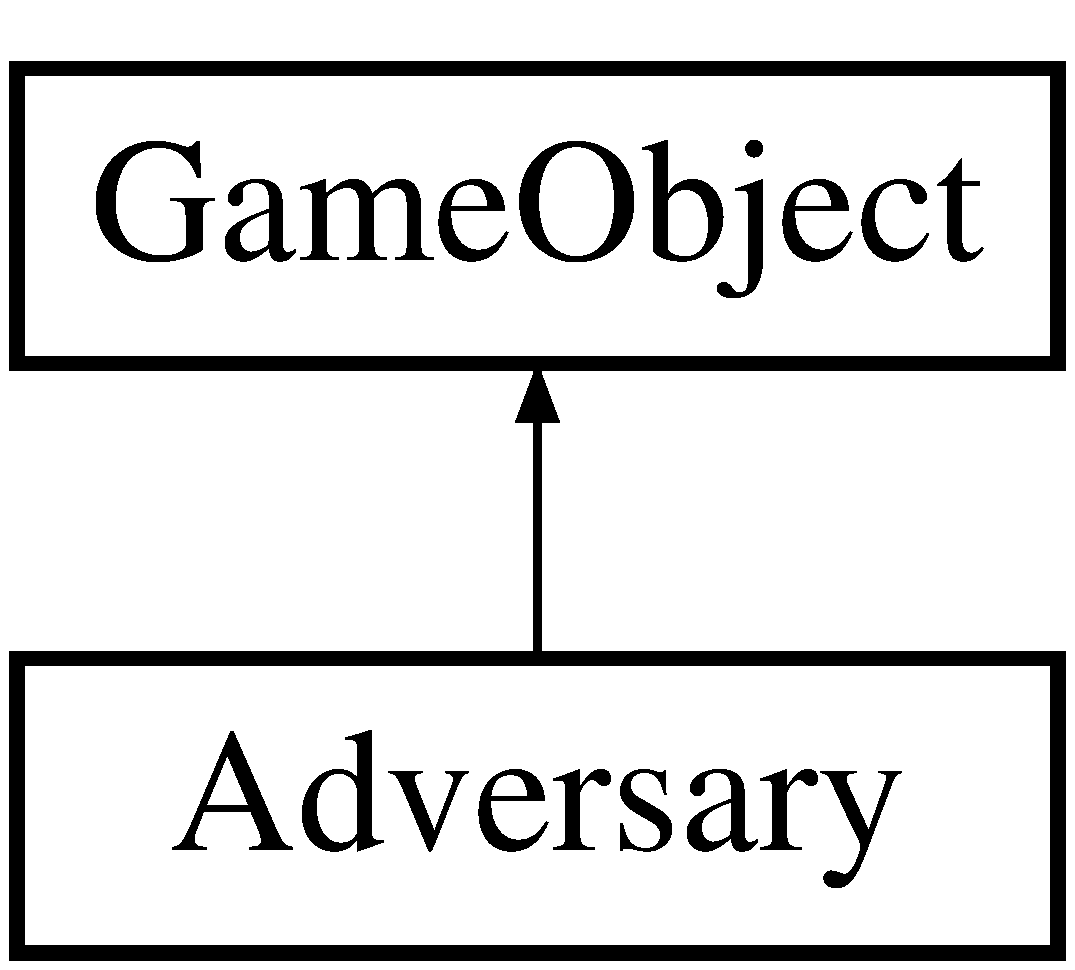
\includegraphics[height=2.000000cm]{class_game_object}
\end{center}
\end{figure}
\subsection*{Public Member Functions}
\begin{DoxyCompactItemize}
\item 
void \hyperlink{class_game_object_a3221e8c7ef7304f94280aca2005a7dd2}{action} (\hyperlink{class_player}{Player} p)
\end{DoxyCompactItemize}


\subsection{Member Function Documentation}
\hypertarget{class_game_object_a3221e8c7ef7304f94280aca2005a7dd2}{}\index{Game\+Object@{Game\+Object}!action@{action}}
\index{action@{action}!Game\+Object@{Game\+Object}}
\subsubsection[{action(\+Player p)}]{\setlength{\rightskip}{0pt plus 5cm}void Game\+Object.\+action (
\begin{DoxyParamCaption}
\item[{{\bf Player}}]{p}
\end{DoxyParamCaption}
)\hspace{0.3cm}{\ttfamily [inline]}}\label{class_game_object_a3221e8c7ef7304f94280aca2005a7dd2}


The documentation for this class was generated from the following file\+:\begin{DoxyCompactItemize}
\item 
src/\hyperlink{_game_object_8java}{Game\+Object.\+java}\end{DoxyCompactItemize}

\hypertarget{interfaceenemy_1_1_enemy_1_1_monster_or_builder}{}\section{enemy.\+Enemy.\+Monster\+Or\+Builder Interface Reference}
\label{interfaceenemy_1_1_enemy_1_1_monster_or_builder}\index{enemy.\+Enemy.\+Monster\+Or\+Builder@{enemy.\+Enemy.\+Monster\+Or\+Builder}}
Inheritance diagram for enemy.\+Enemy.\+Monster\+Or\+Builder\+:\begin{figure}[H]
\begin{center}
\leavevmode
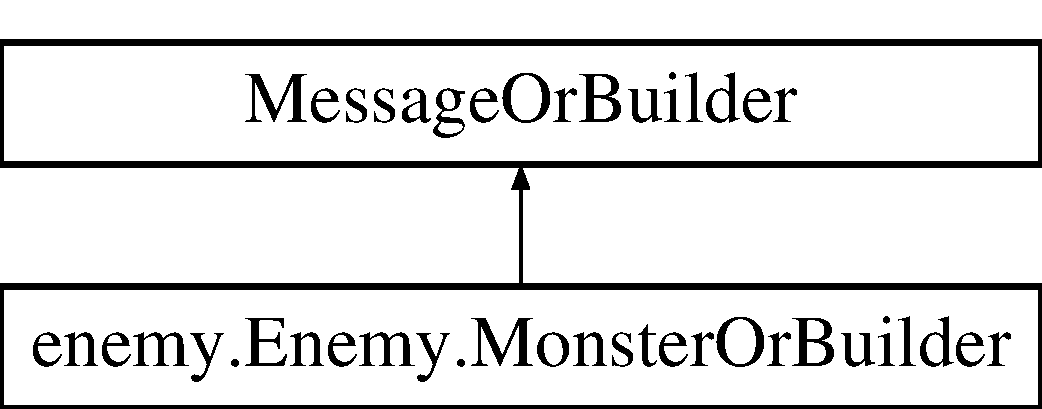
\includegraphics[height=2.000000cm]{interfaceenemy_1_1_enemy_1_1_monster_or_builder}
\end{center}
\end{figure}
\subsection*{Public Member Functions}
\begin{DoxyCompactItemize}
\item 
boolean \hyperlink{interfaceenemy_1_1_enemy_1_1_monster_or_builder_a6b176c6b78d427de79efd20f927a62c8}{has\+Type} ()
\item 
java.\+lang.\+String \hyperlink{interfaceenemy_1_1_enemy_1_1_monster_or_builder_a841aa6c26c499577d603915fd1ac8b41}{get\+Type} ()
\item 
com.\+google.\+protobuf.\+Byte\+String \hyperlink{interfaceenemy_1_1_enemy_1_1_monster_or_builder_adebc3b52131dcbc776b2319af774d1ec}{get\+Type\+Bytes} ()
\item 
boolean \hyperlink{interfaceenemy_1_1_enemy_1_1_monster_or_builder_aab69d054af2dab8ac2ce9f72c4adeaee}{has\+Health} ()
\item 
int \hyperlink{interfaceenemy_1_1_enemy_1_1_monster_or_builder_a8d716340ab45c1c19416e76eb97ea1a6}{get\+Health} ()
\item 
boolean \hyperlink{interfaceenemy_1_1_enemy_1_1_monster_or_builder_a58b07ebaacd518371114e646f2629b68}{has\+Attack} ()
\item 
int \hyperlink{interfaceenemy_1_1_enemy_1_1_monster_or_builder_aa88fa088b2a4a68640345817ed24d54d}{get\+Attack} ()
\item 
boolean \hyperlink{interfaceenemy_1_1_enemy_1_1_monster_or_builder_ab41eec40941a2626b07b61f4ecfdecb3}{has\+Name} ()
\item 
java.\+lang.\+String \hyperlink{interfaceenemy_1_1_enemy_1_1_monster_or_builder_a71db3323eccff3b3dd2788d54178e821}{get\+Name} ()
\item 
com.\+google.\+protobuf.\+Byte\+String \hyperlink{interfaceenemy_1_1_enemy_1_1_monster_or_builder_aae916496b512a0ad203692250dd1ec91}{get\+Name\+Bytes} ()
\end{DoxyCompactItemize}


\subsection{Member Function Documentation}
\hypertarget{interfaceenemy_1_1_enemy_1_1_monster_or_builder_aa88fa088b2a4a68640345817ed24d54d}{}\index{enemy\+::\+Enemy\+::\+Monster\+Or\+Builder@{enemy\+::\+Enemy\+::\+Monster\+Or\+Builder}!get\+Attack@{get\+Attack}}
\index{get\+Attack@{get\+Attack}!enemy\+::\+Enemy\+::\+Monster\+Or\+Builder@{enemy\+::\+Enemy\+::\+Monster\+Or\+Builder}}
\subsubsection[{get\+Attack()}]{\setlength{\rightskip}{0pt plus 5cm}int enemy.\+Enemy.\+Monster\+Or\+Builder.\+get\+Attack (
\begin{DoxyParamCaption}
{}
\end{DoxyParamCaption}
)}\label{interfaceenemy_1_1_enemy_1_1_monster_or_builder_aa88fa088b2a4a68640345817ed24d54d}
{\ttfamily required int32 attack = 3;} \hypertarget{interfaceenemy_1_1_enemy_1_1_monster_or_builder_a8d716340ab45c1c19416e76eb97ea1a6}{}\index{enemy\+::\+Enemy\+::\+Monster\+Or\+Builder@{enemy\+::\+Enemy\+::\+Monster\+Or\+Builder}!get\+Health@{get\+Health}}
\index{get\+Health@{get\+Health}!enemy\+::\+Enemy\+::\+Monster\+Or\+Builder@{enemy\+::\+Enemy\+::\+Monster\+Or\+Builder}}
\subsubsection[{get\+Health()}]{\setlength{\rightskip}{0pt plus 5cm}int enemy.\+Enemy.\+Monster\+Or\+Builder.\+get\+Health (
\begin{DoxyParamCaption}
{}
\end{DoxyParamCaption}
)}\label{interfaceenemy_1_1_enemy_1_1_monster_or_builder_a8d716340ab45c1c19416e76eb97ea1a6}
{\ttfamily required int32 health = 2;} \hypertarget{interfaceenemy_1_1_enemy_1_1_monster_or_builder_a71db3323eccff3b3dd2788d54178e821}{}\index{enemy\+::\+Enemy\+::\+Monster\+Or\+Builder@{enemy\+::\+Enemy\+::\+Monster\+Or\+Builder}!get\+Name@{get\+Name}}
\index{get\+Name@{get\+Name}!enemy\+::\+Enemy\+::\+Monster\+Or\+Builder@{enemy\+::\+Enemy\+::\+Monster\+Or\+Builder}}
\subsubsection[{get\+Name()}]{\setlength{\rightskip}{0pt plus 5cm}java.\+lang.\+String enemy.\+Enemy.\+Monster\+Or\+Builder.\+get\+Name (
\begin{DoxyParamCaption}
{}
\end{DoxyParamCaption}
)}\label{interfaceenemy_1_1_enemy_1_1_monster_or_builder_a71db3323eccff3b3dd2788d54178e821}
{\ttfamily optional string name = 4;} \hypertarget{interfaceenemy_1_1_enemy_1_1_monster_or_builder_aae916496b512a0ad203692250dd1ec91}{}\index{enemy\+::\+Enemy\+::\+Monster\+Or\+Builder@{enemy\+::\+Enemy\+::\+Monster\+Or\+Builder}!get\+Name\+Bytes@{get\+Name\+Bytes}}
\index{get\+Name\+Bytes@{get\+Name\+Bytes}!enemy\+::\+Enemy\+::\+Monster\+Or\+Builder@{enemy\+::\+Enemy\+::\+Monster\+Or\+Builder}}
\subsubsection[{get\+Name\+Bytes()}]{\setlength{\rightskip}{0pt plus 5cm}com.\+google.\+protobuf.\+Byte\+String enemy.\+Enemy.\+Monster\+Or\+Builder.\+get\+Name\+Bytes (
\begin{DoxyParamCaption}
{}
\end{DoxyParamCaption}
)}\label{interfaceenemy_1_1_enemy_1_1_monster_or_builder_aae916496b512a0ad203692250dd1ec91}
{\ttfamily optional string name = 4;} \hypertarget{interfaceenemy_1_1_enemy_1_1_monster_or_builder_a841aa6c26c499577d603915fd1ac8b41}{}\index{enemy\+::\+Enemy\+::\+Monster\+Or\+Builder@{enemy\+::\+Enemy\+::\+Monster\+Or\+Builder}!get\+Type@{get\+Type}}
\index{get\+Type@{get\+Type}!enemy\+::\+Enemy\+::\+Monster\+Or\+Builder@{enemy\+::\+Enemy\+::\+Monster\+Or\+Builder}}
\subsubsection[{get\+Type()}]{\setlength{\rightskip}{0pt plus 5cm}java.\+lang.\+String enemy.\+Enemy.\+Monster\+Or\+Builder.\+get\+Type (
\begin{DoxyParamCaption}
{}
\end{DoxyParamCaption}
)}\label{interfaceenemy_1_1_enemy_1_1_monster_or_builder_a841aa6c26c499577d603915fd1ac8b41}
{\ttfamily required string type = 1;} \hypertarget{interfaceenemy_1_1_enemy_1_1_monster_or_builder_adebc3b52131dcbc776b2319af774d1ec}{}\index{enemy\+::\+Enemy\+::\+Monster\+Or\+Builder@{enemy\+::\+Enemy\+::\+Monster\+Or\+Builder}!get\+Type\+Bytes@{get\+Type\+Bytes}}
\index{get\+Type\+Bytes@{get\+Type\+Bytes}!enemy\+::\+Enemy\+::\+Monster\+Or\+Builder@{enemy\+::\+Enemy\+::\+Monster\+Or\+Builder}}
\subsubsection[{get\+Type\+Bytes()}]{\setlength{\rightskip}{0pt plus 5cm}com.\+google.\+protobuf.\+Byte\+String enemy.\+Enemy.\+Monster\+Or\+Builder.\+get\+Type\+Bytes (
\begin{DoxyParamCaption}
{}
\end{DoxyParamCaption}
)}\label{interfaceenemy_1_1_enemy_1_1_monster_or_builder_adebc3b52131dcbc776b2319af774d1ec}
{\ttfamily required string type = 1;} \hypertarget{interfaceenemy_1_1_enemy_1_1_monster_or_builder_a58b07ebaacd518371114e646f2629b68}{}\index{enemy\+::\+Enemy\+::\+Monster\+Or\+Builder@{enemy\+::\+Enemy\+::\+Monster\+Or\+Builder}!has\+Attack@{has\+Attack}}
\index{has\+Attack@{has\+Attack}!enemy\+::\+Enemy\+::\+Monster\+Or\+Builder@{enemy\+::\+Enemy\+::\+Monster\+Or\+Builder}}
\subsubsection[{has\+Attack()}]{\setlength{\rightskip}{0pt plus 5cm}boolean enemy.\+Enemy.\+Monster\+Or\+Builder.\+has\+Attack (
\begin{DoxyParamCaption}
{}
\end{DoxyParamCaption}
)}\label{interfaceenemy_1_1_enemy_1_1_monster_or_builder_a58b07ebaacd518371114e646f2629b68}
{\ttfamily required int32 attack = 3;} \hypertarget{interfaceenemy_1_1_enemy_1_1_monster_or_builder_aab69d054af2dab8ac2ce9f72c4adeaee}{}\index{enemy\+::\+Enemy\+::\+Monster\+Or\+Builder@{enemy\+::\+Enemy\+::\+Monster\+Or\+Builder}!has\+Health@{has\+Health}}
\index{has\+Health@{has\+Health}!enemy\+::\+Enemy\+::\+Monster\+Or\+Builder@{enemy\+::\+Enemy\+::\+Monster\+Or\+Builder}}
\subsubsection[{has\+Health()}]{\setlength{\rightskip}{0pt plus 5cm}boolean enemy.\+Enemy.\+Monster\+Or\+Builder.\+has\+Health (
\begin{DoxyParamCaption}
{}
\end{DoxyParamCaption}
)}\label{interfaceenemy_1_1_enemy_1_1_monster_or_builder_aab69d054af2dab8ac2ce9f72c4adeaee}
{\ttfamily required int32 health = 2;} \hypertarget{interfaceenemy_1_1_enemy_1_1_monster_or_builder_ab41eec40941a2626b07b61f4ecfdecb3}{}\index{enemy\+::\+Enemy\+::\+Monster\+Or\+Builder@{enemy\+::\+Enemy\+::\+Monster\+Or\+Builder}!has\+Name@{has\+Name}}
\index{has\+Name@{has\+Name}!enemy\+::\+Enemy\+::\+Monster\+Or\+Builder@{enemy\+::\+Enemy\+::\+Monster\+Or\+Builder}}
\subsubsection[{has\+Name()}]{\setlength{\rightskip}{0pt plus 5cm}boolean enemy.\+Enemy.\+Monster\+Or\+Builder.\+has\+Name (
\begin{DoxyParamCaption}
{}
\end{DoxyParamCaption}
)}\label{interfaceenemy_1_1_enemy_1_1_monster_or_builder_ab41eec40941a2626b07b61f4ecfdecb3}
{\ttfamily optional string name = 4;} \hypertarget{interfaceenemy_1_1_enemy_1_1_monster_or_builder_a6b176c6b78d427de79efd20f927a62c8}{}\index{enemy\+::\+Enemy\+::\+Monster\+Or\+Builder@{enemy\+::\+Enemy\+::\+Monster\+Or\+Builder}!has\+Type@{has\+Type}}
\index{has\+Type@{has\+Type}!enemy\+::\+Enemy\+::\+Monster\+Or\+Builder@{enemy\+::\+Enemy\+::\+Monster\+Or\+Builder}}
\subsubsection[{has\+Type()}]{\setlength{\rightskip}{0pt plus 5cm}boolean enemy.\+Enemy.\+Monster\+Or\+Builder.\+has\+Type (
\begin{DoxyParamCaption}
{}
\end{DoxyParamCaption}
)}\label{interfaceenemy_1_1_enemy_1_1_monster_or_builder_a6b176c6b78d427de79efd20f927a62c8}
{\ttfamily required string type = 1;} 

The documentation for this interface was generated from the following file\+:\begin{DoxyCompactItemize}
\item 
src/protobuf/\hyperlink{_enemy_8java}{Enemy.\+java}\end{DoxyCompactItemize}

\hypertarget{class_player}{}\section{Player Class Reference}
\label{class_player}\index{Player@{Player}}
\subsection*{Public Member Functions}
\begin{DoxyCompactItemize}
\item 
\hyperlink{class_player_a712a726b07cf901c040116d6d0c5cc66}{Player} ()
\item 
void \hyperlink{class_player_aa0bda57e73a788eee38fa3837b661a0c}{use\+Potion} ()
\end{DoxyCompactItemize}
\subsection*{Public Attributes}
\begin{DoxyCompactItemize}
\item 
int \hyperlink{class_player_ab064f330cef84e2e062fd6446db24184}{health}
\item 
int \hyperlink{class_player_a9912e57826c51a067ab34db854f31562}{attack}
\item 
int \hyperlink{class_player_a572d7dffbbd9d958c88b1aa160317fee}{potion}
\end{DoxyCompactItemize}


\subsection{Constructor \& Destructor Documentation}
\hypertarget{class_player_a712a726b07cf901c040116d6d0c5cc66}{}\index{Player@{Player}!Player@{Player}}
\index{Player@{Player}!Player@{Player}}
\subsubsection[{Player()}]{\setlength{\rightskip}{0pt plus 5cm}Player.\+Player (
\begin{DoxyParamCaption}
{}
\end{DoxyParamCaption}
)\hspace{0.3cm}{\ttfamily [inline]}}\label{class_player_a712a726b07cf901c040116d6d0c5cc66}


\subsection{Member Function Documentation}
\hypertarget{class_player_aa0bda57e73a788eee38fa3837b661a0c}{}\index{Player@{Player}!use\+Potion@{use\+Potion}}
\index{use\+Potion@{use\+Potion}!Player@{Player}}
\subsubsection[{use\+Potion()}]{\setlength{\rightskip}{0pt plus 5cm}void Player.\+use\+Potion (
\begin{DoxyParamCaption}
{}
\end{DoxyParamCaption}
)\hspace{0.3cm}{\ttfamily [inline]}}\label{class_player_aa0bda57e73a788eee38fa3837b661a0c}


\subsection{Member Data Documentation}
\hypertarget{class_player_a9912e57826c51a067ab34db854f31562}{}\index{Player@{Player}!attack@{attack}}
\index{attack@{attack}!Player@{Player}}
\subsubsection[{attack}]{\setlength{\rightskip}{0pt plus 5cm}int Player.\+attack}\label{class_player_a9912e57826c51a067ab34db854f31562}
\hypertarget{class_player_ab064f330cef84e2e062fd6446db24184}{}\index{Player@{Player}!health@{health}}
\index{health@{health}!Player@{Player}}
\subsubsection[{health}]{\setlength{\rightskip}{0pt plus 5cm}int Player.\+health}\label{class_player_ab064f330cef84e2e062fd6446db24184}
\hypertarget{class_player_a572d7dffbbd9d958c88b1aa160317fee}{}\index{Player@{Player}!potion@{potion}}
\index{potion@{potion}!Player@{Player}}
\subsubsection[{potion}]{\setlength{\rightskip}{0pt plus 5cm}int Player.\+potion}\label{class_player_a572d7dffbbd9d958c88b1aa160317fee}


The documentation for this class was generated from the following file\+:\begin{DoxyCompactItemize}
\item 
src/\hyperlink{_player_8java}{Player.\+java}\end{DoxyCompactItemize}

\hypertarget{class_room}{}\section{Room Class Reference}
\label{class_room}\index{Room@{Room}}
\subsection*{Public Member Functions}
\begin{DoxyCompactItemize}
\item 
\hyperlink{class_room_aca38f1673fd9264e15575e6faa34ba44}{Room} ()
\item 
void \hyperlink{class_room_a5736252d41ba0dd28448a8a503ffac6b}{list\+Objects\+In\+Room} ()
\item 
\hyperlink{class_room_aca38f1673fd9264e15575e6faa34ba44}{Room} ()
\item 
\hyperlink{class_room_a7f6ed8f23c70b90599acdd68ca7aed06}{Room} (List$<$ \hyperlink{class_room}{Room} $>$ neighboring\+Rooms)
\item 
void \hyperlink{class_room_a4f262a8900dd0bed2891f3c21e1baa0f}{print\+List\+Objects\+In\+Room} (String prefix, String postfix, String delimiter)
\item 
void \hyperlink{class_room_a5736252d41ba0dd28448a8a503ffac6b}{list\+Objects\+In\+Room} ()
\item 
void \hyperlink{class_room_af0380bf1a3f1ef06242b8db7dee85567}{initiate\+Events} (\hyperlink{class_player}{Player} p)
\end{DoxyCompactItemize}


\subsection{Detailed Description}
\hyperlink{class_room}{Room} is the class representation of any space in the game. A \hyperlink{class_room}{Room} object encapsulates the state information needed for the various configurations of of games.

\begin{DoxyAuthor}{Author}
... 

Richard B. Wagner 
\end{DoxyAuthor}


\subsection{Constructor \& Destructor Documentation}
\hypertarget{class_room_aca38f1673fd9264e15575e6faa34ba44}{}\index{Room@{Room}!Room@{Room}}
\index{Room@{Room}!Room@{Room}}
\subsubsection[{Room()}]{\setlength{\rightskip}{0pt plus 5cm}Room.\+Room (
\begin{DoxyParamCaption}
{}
\end{DoxyParamCaption}
)\hspace{0.3cm}{\ttfamily [inline]}}\label{class_room_aca38f1673fd9264e15575e6faa34ba44}
\hypertarget{class_room_aca38f1673fd9264e15575e6faa34ba44}{}\index{Room@{Room}!Room@{Room}}
\index{Room@{Room}!Room@{Room}}
\subsubsection[{Room()}]{\setlength{\rightskip}{0pt plus 5cm}Room.\+Room (
\begin{DoxyParamCaption}
{}
\end{DoxyParamCaption}
)\hspace{0.3cm}{\ttfamily [inline]}}\label{class_room_aca38f1673fd9264e15575e6faa34ba44}
Default constructor. (For invocation by subclass constructors, typically implicit.) \hypertarget{class_room_a7f6ed8f23c70b90599acdd68ca7aed06}{}\index{Room@{Room}!Room@{Room}}
\index{Room@{Room}!Room@{Room}}
\subsubsection[{Room(\+List$<$ Room $>$ neighboring\+Rooms)}]{\setlength{\rightskip}{0pt plus 5cm}Room.\+Room (
\begin{DoxyParamCaption}
\item[{List$<$ {\bf Room} $>$}]{neighboring\+Rooms}
\end{DoxyParamCaption}
)\hspace{0.3cm}{\ttfamily [inline]}}\label{class_room_a7f6ed8f23c70b90599acdd68ca7aed06}
Constructor 

\subsection{Member Function Documentation}
\hypertarget{class_room_af0380bf1a3f1ef06242b8db7dee85567}{}\index{Room@{Room}!initiate\+Events@{initiate\+Events}}
\index{initiate\+Events@{initiate\+Events}!Room@{Room}}
\subsubsection[{initiate\+Events(\+Player p)}]{\setlength{\rightskip}{0pt plus 5cm}void Room.\+initiate\+Events (
\begin{DoxyParamCaption}
\item[{{\bf Player}}]{p}
\end{DoxyParamCaption}
)\hspace{0.3cm}{\ttfamily [inline]}}\label{class_room_af0380bf1a3f1ef06242b8db7dee85567}
For each \hyperlink{class_game_object}{Game\+Object} in the room, call that objects action method. For items, this will be an empty call. \hypertarget{class_room_a5736252d41ba0dd28448a8a503ffac6b}{}\index{Room@{Room}!list\+Objects\+In\+Room@{list\+Objects\+In\+Room}}
\index{list\+Objects\+In\+Room@{list\+Objects\+In\+Room}!Room@{Room}}
\subsubsection[{list\+Objects\+In\+Room()}]{\setlength{\rightskip}{0pt plus 5cm}void Room.\+list\+Objects\+In\+Room (
\begin{DoxyParamCaption}
{}
\end{DoxyParamCaption}
)\hspace{0.3cm}{\ttfamily [inline]}}\label{class_room_a5736252d41ba0dd28448a8a503ffac6b}
\hypertarget{class_room_a5736252d41ba0dd28448a8a503ffac6b}{}\index{Room@{Room}!list\+Objects\+In\+Room@{list\+Objects\+In\+Room}}
\index{list\+Objects\+In\+Room@{list\+Objects\+In\+Room}!Room@{Room}}
\subsubsection[{list\+Objects\+In\+Room()}]{\setlength{\rightskip}{0pt plus 5cm}void Room.\+list\+Objects\+In\+Room (
\begin{DoxyParamCaption}
{}
\end{DoxyParamCaption}
)\hspace{0.3cm}{\ttfamily [inline]}}\label{class_room_a5736252d41ba0dd28448a8a503ffac6b}
Prints a list of the \hyperlink{class_game_object}{Game\+Object} in a room. 
\begin{DoxyParams}{Parameters}
{\em prefix} & a String to prepend at the beginning the output \\
\hline
{\em postfix} & a String to append at the end of the output \\
\hline
{\em delimiter} & a string to insert in between each element in the list \\
\hline
\end{DoxyParams}
\hypertarget{class_room_a4f262a8900dd0bed2891f3c21e1baa0f}{}\index{Room@{Room}!print\+List\+Objects\+In\+Room@{print\+List\+Objects\+In\+Room}}
\index{print\+List\+Objects\+In\+Room@{print\+List\+Objects\+In\+Room}!Room@{Room}}
\subsubsection[{print\+List\+Objects\+In\+Room(\+String prefix, String postfix, String delimiter)}]{\setlength{\rightskip}{0pt plus 5cm}void Room.\+print\+List\+Objects\+In\+Room (
\begin{DoxyParamCaption}
\item[{String}]{prefix, }
\item[{String}]{postfix, }
\item[{String}]{delimiter}
\end{DoxyParamCaption}
)\hspace{0.3cm}{\ttfamily [inline]}}\label{class_room_a4f262a8900dd0bed2891f3c21e1baa0f}
Prints a list of the \hyperlink{class_game_object}{Game\+Object} in a room. 
\begin{DoxyParams}{Parameters}
{\em prefix} & a String to prepend at the beginning the output \\
\hline
{\em postfix} & a String to append at the end of the output \\
\hline
{\em delimiter} & a string to insert in between each element in the list \\
\hline
\end{DoxyParams}


The documentation for this class was generated from the following file\+:\begin{DoxyCompactItemize}
\item 
other/project\+\_\+phase3/\hyperlink{other_2project__phase3_2_room_8java}{Room.\+java}\end{DoxyCompactItemize}

\hypertarget{class_test_bed1}{}\section{Test\+Bed1 Class Reference}
\label{class_test_bed1}\index{Test\+Bed1@{Test\+Bed1}}
\subsection*{Static Public Member Functions}
\begin{DoxyCompactItemize}
\item 
static void \hyperlink{class_test_bed1_af5005ddaffb3a19a4f69ebdae1385252}{main} (String\mbox{[}$\,$\mbox{]} args)
\end{DoxyCompactItemize}


\subsection{Detailed Description}
This class is just to test \begin{DoxyAuthor}{Author}
breckwagner 
\end{DoxyAuthor}


\subsection{Member Function Documentation}
\hypertarget{class_test_bed1_af5005ddaffb3a19a4f69ebdae1385252}{}\index{Test\+Bed1@{Test\+Bed1}!main@{main}}
\index{main@{main}!Test\+Bed1@{Test\+Bed1}}
\subsubsection[{main(\+String[] args)}]{\setlength{\rightskip}{0pt plus 5cm}static void Test\+Bed1.\+main (
\begin{DoxyParamCaption}
\item[{String\mbox{[}$\,$\mbox{]}}]{args}
\end{DoxyParamCaption}
)\hspace{0.3cm}{\ttfamily [inline]}, {\ttfamily [static]}}\label{class_test_bed1_af5005ddaffb3a19a4f69ebdae1385252}

\begin{DoxyParams}{Parameters}
{\em args} & \\
\hline
\end{DoxyParams}


The documentation for this class was generated from the following file\+:\begin{DoxyCompactItemize}
\item 
src/\hyperlink{_test_bed1_8java}{Test\+Bed1.\+java}\end{DoxyCompactItemize}

\hypertarget{class_test_cases}{}\section{Test\+Cases Class Reference}
\label{class_test_cases}\index{Test\+Cases@{Test\+Cases}}
\subsection*{Public Member Functions}
\begin{DoxyCompactItemize}
\item 
void \hyperlink{class_test_cases_a459e020aabe6b8422d92ad0f9132ff9b}{test\+Player\+Health} ()
\end{DoxyCompactItemize}


\subsection{Member Function Documentation}
\hypertarget{class_test_cases_a459e020aabe6b8422d92ad0f9132ff9b}{}\index{Test\+Cases@{Test\+Cases}!test\+Player\+Health@{test\+Player\+Health}}
\index{test\+Player\+Health@{test\+Player\+Health}!Test\+Cases@{Test\+Cases}}
\subsubsection[{test\+Player\+Health()}]{\setlength{\rightskip}{0pt plus 5cm}void Test\+Cases.\+test\+Player\+Health (
\begin{DoxyParamCaption}
{}
\end{DoxyParamCaption}
)\hspace{0.3cm}{\ttfamily [inline]}}\label{class_test_cases_a459e020aabe6b8422d92ad0f9132ff9b}


The documentation for this class was generated from the following file\+:\begin{DoxyCompactItemize}
\item 
src/\hyperlink{_test_cases_8java}{Test\+Cases.\+java}\end{DoxyCompactItemize}

\hypertarget{interfaceenemy_1_1_enemy_1_1_trap_or_builder}{}\section{enemy.\+Enemy.\+Trap\+Or\+Builder Interface Reference}
\label{interfaceenemy_1_1_enemy_1_1_trap_or_builder}\index{enemy.\+Enemy.\+Trap\+Or\+Builder@{enemy.\+Enemy.\+Trap\+Or\+Builder}}
Inheritance diagram for enemy.\+Enemy.\+Trap\+Or\+Builder\+:\begin{figure}[H]
\begin{center}
\leavevmode
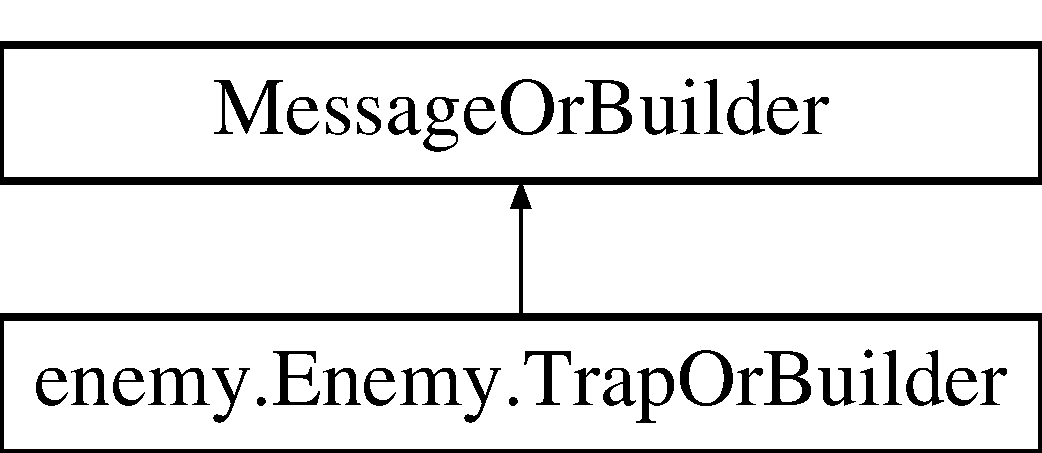
\includegraphics[height=2.000000cm]{interfaceenemy_1_1_enemy_1_1_trap_or_builder}
\end{center}
\end{figure}
\subsection*{Public Member Functions}
\begin{DoxyCompactItemize}
\item 
boolean \hyperlink{interfaceenemy_1_1_enemy_1_1_trap_or_builder_ab31536f63dbd1ece8c0a84c049cd4794}{has\+Attack} ()
\item 
int \hyperlink{interfaceenemy_1_1_enemy_1_1_trap_or_builder_ac619469470cc8f5e7121e1402be7d6da}{get\+Attack} ()
\item 
boolean \hyperlink{interfaceenemy_1_1_enemy_1_1_trap_or_builder_a59cfd22dba9c70bc5f87b235fb37763f}{has\+Name} ()
\item 
java.\+lang.\+String \hyperlink{interfaceenemy_1_1_enemy_1_1_trap_or_builder_ad79bd02341bb3d69bf66f75015f703c7}{get\+Name} ()
\item 
com.\+google.\+protobuf.\+Byte\+String \hyperlink{interfaceenemy_1_1_enemy_1_1_trap_or_builder_aaeed7f889fca017da08fc3d03b4c2e2d}{get\+Name\+Bytes} ()
\end{DoxyCompactItemize}


\subsection{Member Function Documentation}
\hypertarget{interfaceenemy_1_1_enemy_1_1_trap_or_builder_ac619469470cc8f5e7121e1402be7d6da}{}\index{enemy\+::\+Enemy\+::\+Trap\+Or\+Builder@{enemy\+::\+Enemy\+::\+Trap\+Or\+Builder}!get\+Attack@{get\+Attack}}
\index{get\+Attack@{get\+Attack}!enemy\+::\+Enemy\+::\+Trap\+Or\+Builder@{enemy\+::\+Enemy\+::\+Trap\+Or\+Builder}}
\subsubsection[{get\+Attack()}]{\setlength{\rightskip}{0pt plus 5cm}int enemy.\+Enemy.\+Trap\+Or\+Builder.\+get\+Attack (
\begin{DoxyParamCaption}
{}
\end{DoxyParamCaption}
)}\label{interfaceenemy_1_1_enemy_1_1_trap_or_builder_ac619469470cc8f5e7121e1402be7d6da}
{\ttfamily required int32 attack = 1;} \hypertarget{interfaceenemy_1_1_enemy_1_1_trap_or_builder_ad79bd02341bb3d69bf66f75015f703c7}{}\index{enemy\+::\+Enemy\+::\+Trap\+Or\+Builder@{enemy\+::\+Enemy\+::\+Trap\+Or\+Builder}!get\+Name@{get\+Name}}
\index{get\+Name@{get\+Name}!enemy\+::\+Enemy\+::\+Trap\+Or\+Builder@{enemy\+::\+Enemy\+::\+Trap\+Or\+Builder}}
\subsubsection[{get\+Name()}]{\setlength{\rightskip}{0pt plus 5cm}java.\+lang.\+String enemy.\+Enemy.\+Trap\+Or\+Builder.\+get\+Name (
\begin{DoxyParamCaption}
{}
\end{DoxyParamCaption}
)}\label{interfaceenemy_1_1_enemy_1_1_trap_or_builder_ad79bd02341bb3d69bf66f75015f703c7}
{\ttfamily optional string name = 2;} \hypertarget{interfaceenemy_1_1_enemy_1_1_trap_or_builder_aaeed7f889fca017da08fc3d03b4c2e2d}{}\index{enemy\+::\+Enemy\+::\+Trap\+Or\+Builder@{enemy\+::\+Enemy\+::\+Trap\+Or\+Builder}!get\+Name\+Bytes@{get\+Name\+Bytes}}
\index{get\+Name\+Bytes@{get\+Name\+Bytes}!enemy\+::\+Enemy\+::\+Trap\+Or\+Builder@{enemy\+::\+Enemy\+::\+Trap\+Or\+Builder}}
\subsubsection[{get\+Name\+Bytes()}]{\setlength{\rightskip}{0pt plus 5cm}com.\+google.\+protobuf.\+Byte\+String enemy.\+Enemy.\+Trap\+Or\+Builder.\+get\+Name\+Bytes (
\begin{DoxyParamCaption}
{}
\end{DoxyParamCaption}
)}\label{interfaceenemy_1_1_enemy_1_1_trap_or_builder_aaeed7f889fca017da08fc3d03b4c2e2d}
{\ttfamily optional string name = 2;} \hypertarget{interfaceenemy_1_1_enemy_1_1_trap_or_builder_ab31536f63dbd1ece8c0a84c049cd4794}{}\index{enemy\+::\+Enemy\+::\+Trap\+Or\+Builder@{enemy\+::\+Enemy\+::\+Trap\+Or\+Builder}!has\+Attack@{has\+Attack}}
\index{has\+Attack@{has\+Attack}!enemy\+::\+Enemy\+::\+Trap\+Or\+Builder@{enemy\+::\+Enemy\+::\+Trap\+Or\+Builder}}
\subsubsection[{has\+Attack()}]{\setlength{\rightskip}{0pt plus 5cm}boolean enemy.\+Enemy.\+Trap\+Or\+Builder.\+has\+Attack (
\begin{DoxyParamCaption}
{}
\end{DoxyParamCaption}
)}\label{interfaceenemy_1_1_enemy_1_1_trap_or_builder_ab31536f63dbd1ece8c0a84c049cd4794}
{\ttfamily required int32 attack = 1;} \hypertarget{interfaceenemy_1_1_enemy_1_1_trap_or_builder_a59cfd22dba9c70bc5f87b235fb37763f}{}\index{enemy\+::\+Enemy\+::\+Trap\+Or\+Builder@{enemy\+::\+Enemy\+::\+Trap\+Or\+Builder}!has\+Name@{has\+Name}}
\index{has\+Name@{has\+Name}!enemy\+::\+Enemy\+::\+Trap\+Or\+Builder@{enemy\+::\+Enemy\+::\+Trap\+Or\+Builder}}
\subsubsection[{has\+Name()}]{\setlength{\rightskip}{0pt plus 5cm}boolean enemy.\+Enemy.\+Trap\+Or\+Builder.\+has\+Name (
\begin{DoxyParamCaption}
{}
\end{DoxyParamCaption}
)}\label{interfaceenemy_1_1_enemy_1_1_trap_or_builder_a59cfd22dba9c70bc5f87b235fb37763f}
{\ttfamily optional string name = 2;} 

The documentation for this interface was generated from the following file\+:\begin{DoxyCompactItemize}
\item 
src/protobuf/\hyperlink{_enemy_8java}{Enemy.\+java}\end{DoxyCompactItemize}

\chapter{File Documentation}
\hypertarget{_i_n_s_t_a_l_l_8md}{}\section{I\+N\+S\+T\+A\+L\+L.\+md File Reference}
\label{_i_n_s_t_a_l_l_8md}\index{I\+N\+S\+T\+A\+L\+L.\+md@{I\+N\+S\+T\+A\+L\+L.\+md}}

\hypertarget{other_2project__phase3_2_room_8java}{}\section{other/project\+\_\+phase3/\+Room.java File Reference}
\label{other_2project__phase3_2_room_8java}\index{other/project\+\_\+phase3/\+Room.\+java@{other/project\+\_\+phase3/\+Room.\+java}}
\subsection*{Classes}
\begin{DoxyCompactItemize}
\item 
class \hyperlink{class_room}{Room}
\end{DoxyCompactItemize}

\hypertarget{src_2_room_8java}{}\section{src/\+Room.java File Reference}
\label{src_2_room_8java}\index{src/\+Room.\+java@{src/\+Room.\+java}}
\subsection*{Classes}
\begin{DoxyCompactItemize}
\item 
class \hyperlink{class_room}{Room}
\end{DoxyCompactItemize}

\hypertarget{_r_e_a_d_m_e_8md}{}\section{R\+E\+A\+D\+M\+E.\+md File Reference}
\label{_r_e_a_d_m_e_8md}\index{R\+E\+A\+D\+M\+E.\+md@{R\+E\+A\+D\+M\+E.\+md}}

\hypertarget{_adversary_8java}{}\section{src/\+Adversary.java File Reference}
\label{_adversary_8java}\index{src/\+Adversary.\+java@{src/\+Adversary.\+java}}
\subsection*{Classes}
\begin{DoxyCompactItemize}
\item 
class \hyperlink{class_adversary}{Adversary}
\end{DoxyCompactItemize}

\hypertarget{_driver_8java}{}\section{src/\+Driver.java File Reference}
\label{_driver_8java}\index{src/\+Driver.\+java@{src/\+Driver.\+java}}
\subsection*{Classes}
\begin{DoxyCompactItemize}
\item 
class \hyperlink{class_driver}{Driver}
\end{DoxyCompactItemize}

\hypertarget{_game_8java}{}\section{src/\+Game.java File Reference}
\label{_game_8java}\index{src/\+Game.\+java@{src/\+Game.\+java}}
\subsection*{Classes}
\begin{DoxyCompactItemize}
\item 
class \hyperlink{class_game}{Game}
\end{DoxyCompactItemize}

\hypertarget{_game_object_8java}{}\section{src/\+Game\+Object.java File Reference}
\label{_game_object_8java}\index{src/\+Game\+Object.\+java@{src/\+Game\+Object.\+java}}
\subsection*{Classes}
\begin{DoxyCompactItemize}
\item 
class \hyperlink{class_game_object}{Game\+Object}
\end{DoxyCompactItemize}

\hypertarget{_player_8java}{}\section{src/\+Player.java File Reference}
\label{_player_8java}\index{src/\+Player.\+java@{src/\+Player.\+java}}
\subsection*{Classes}
\begin{DoxyCompactItemize}
\item 
class \hyperlink{class_player}{Player}
\end{DoxyCompactItemize}

\hypertarget{_enemy_8java}{}\section{src/protobuf/\+Enemy.java File Reference}
\label{_enemy_8java}\index{src/protobuf/\+Enemy.\+java@{src/protobuf/\+Enemy.\+java}}
\subsection*{Classes}
\begin{DoxyCompactItemize}
\item 
class \hyperlink{classenemy_1_1_enemy}{enemy.\+Enemy}
\item 
interface \hyperlink{interfaceenemy_1_1_enemy_1_1_monster_or_builder}{enemy.\+Enemy.\+Monster\+Or\+Builder}
\item 
class {\bfseries enemy.\+Enemy.\+Monster}
\item 
class {\bfseries enemy.\+Enemy.\+Monster.\+Builder}
\item 
interface \hyperlink{interfaceenemy_1_1_enemy_1_1_trap_or_builder}{enemy.\+Enemy.\+Trap\+Or\+Builder}
\item 
class {\bfseries enemy.\+Enemy.\+Trap}
\item 
class {\bfseries enemy.\+Enemy.\+Trap.\+Builder}
\end{DoxyCompactItemize}
\subsection*{Packages}
\begin{DoxyCompactItemize}
\item 
package \hyperlink{namespaceenemy}{enemy}
\end{DoxyCompactItemize}

\hypertarget{_test_bed1_8java}{}\section{src/\+Test\+Bed1.java File Reference}
\label{_test_bed1_8java}\index{src/\+Test\+Bed1.\+java@{src/\+Test\+Bed1.\+java}}
\subsection*{Classes}
\begin{DoxyCompactItemize}
\item 
class \hyperlink{class_test_bed1}{Test\+Bed1}
\end{DoxyCompactItemize}

\hypertarget{_test_cases_8java}{}\section{src/\+Test\+Cases.java File Reference}
\label{_test_cases_8java}\index{src/\+Test\+Cases.\+java@{src/\+Test\+Cases.\+java}}
\subsection*{Classes}
\begin{DoxyCompactItemize}
\item 
class \hyperlink{class_test_cases}{Test\+Cases}
\end{DoxyCompactItemize}

\hypertarget{_world_builder_8java}{}\section{src/\+World\+Builder.java File Reference}
\label{_world_builder_8java}\index{src/\+World\+Builder.\+java@{src/\+World\+Builder.\+java}}
\subsection*{Classes}
\begin{DoxyCompactItemize}
\item 
class {\bfseries World\+Builder}
\end{DoxyCompactItemize}

%--- End generated contents ---

% Index
\backmatter
\newpage
\phantomsection
\clearemptydoublepage
\addcontentsline{toc}{chapter}{Index}
\printindex

\end{document}
